% https://tex.stackexchange.com/questions/144577/remove-chapter-number-from-bibliography

\documentclass[
%a4paper, 
11pt, 
ngerman,
listof=totocnumbered,
oneside,
%bibliography=totoc,
bibliography=totocnumbered,
abstracton
]{scrreprt}

\usepackage[T1]{fontenc}
\usepackage[utf8]{inputenc}
\usepackage[ngerman]{babel}
\usepackage{graphicx}
\usepackage{lipsum}
\usepackage{csquotes}
\usepackage[onehalfspacing]{setspace}
\usepackage{subcaption}
\usepackage{scrlayer-scrpage}
\usepackage{float}
\usepackage{mhchem}
\usepackage{siunitx}
\usepackage{pdfpages}
\chead*{\pagemark}
\cofoot*{}

\usepackage{lineno}
%\usepackage{layout}
%
%\makeatletter
%\renewcommand*{\lay@value}[2]{%
%	\strip@pt\dimexpr0.351459\dimexpr\csname#2\endcsname\relax\relax mm%
%}
%\makeatother

\makeatletter
\newcommand \Dotfill {\leavevmode \cleaders \hb@xt@ .22em{\hss .\hss }\hfill \kern \z@}
\makeatother

\usepackage[a4paper
%,showframe
,top=1.1cm
,bottom=2.5cm
,left=3.5cm
,right=2.5cm
,headsep=0.775cm, 
,headheight=0.625cm, 
%,top=1.2cm 1.2 + .75 + 1.05 = 3; 3.5 = 1.225 + 0.875 + 1.4; 2.5 = 1 + .625 + .875
,includehead
%,headskip=1.25cm
]{geometry}

\usepackage[
backend=biber,
style=authoryear-ibid,
%sorting=ynt
]{biblatex}
\addbibresource{gravitropismus-bibliography.bib}

\title{Untersuchung von Gravitropismus bei \emph{Lepidium sativum} mit einem selbstgebauten Klinostat unter Zimmerbedingungen}

\subtitle{W-Seminararbeit im Fach Biologie am Luitpold-Gymnasium München}

\author{Alexandra Smirnova}


\begin{document}
	

\includepdf[pages={1}]{2.pdf}

\begingroup
\renewcommand*{\chapterpagestyle}{empty}
\pagestyle{empty}
% \maketitle
\tableofcontents
\clearpage
\endgroup
	
\renewcommand\abstractname{Abstract}
\begin{abstract}

Gravitropismus ist seit dem 19. Jahrhundert als naturwissenschaftliches Phänomen bekannt. Pflanzen orientieren sich an der Schwerkraft, um in Richtung von Nährstoffen ({\glqq nach unten\grqq}) wachsen zu können. Die dafür verantwortlichen Mechanismen stellen ein aktuelles Forschungsgebiet dar und bilden die Grundlage der vorliegenden Arbeit. 

Zunächst wird eine fachliche Analyse der Thematik Gravitropismus durchgeführt. Dabei werden grundlegende Begriffe eingeführt und anschließend auf die Reizaufnahme bei Pflanzen sowie auf die pflanzliche Signaltransduktion und das differenzielle Wachstum eingegangen. 

Im praktischen Teil der Arbeit erfolgt der experimentelle Nachweis von Gravitropismus bei \emph{Lepidium sativum} unter Haushaltsbedingungen; hierfür wird ein selbstständig konstruierter Klinostat verwendet. Das erfolgreich durchgeführte Experiment wird beschrieben und die Ergebnisse aufgearbeitet. 

Abschließend wird auf die Bedeutung von Gravitropismus eingegangen und es werden mögliche weiterführende experimentelle Ansätze in einem Ausblick diskutiert. 
	
\end{abstract}

% \let\raggedsection\centering
% \section*{\abstractname}
% Dies ist die Zusammenfassung auf Deutsch.

\chapter{Gravitropismus als wichtige Pflanzeneigenschaft}

Viele Pflanzen sind an die Erde festgebundene Organismen, die ab ihrer Keimung ihr ganzes Leben an einem Ort verbringen. Wurzeln verankern die Pflanzen an die Erde und versorgen sie mit Mineralionen und Wasser. Sprossen dagegen wachsen oberhalb der Erde, wo sie Photosynthese betreiben können. Wurzeln und Sprossen orientieren sich während dem Wachstum unter anderem an der Schwerkraft---diese Fähigkeit wird als Gravitropismus bezeichnet \parencite[2]{Masson2002}. 

Gravitropismus wurde vor zweihundert Jahren als biologisches Phänomen anerkannt und bleibt bis heute ein aktiver Forschungsbereich, was auch an der Vielzahl der wissenschaftlichen Veröffentlichungen erkennbar ist. Zum Beispiel beschäftigt sich eine Gruppe von Naturwissenschaftlern mit Gravitropismus in Bezug auf die Landwirtschaft, um das Potenzial der Pflanze auszuschöpfen. Gravitropismus ist dafür verantwortlich, dass sich das Gewächs nach einem Unwetter wieder aufrichtet und weiter wächst \parencite[343]{Chen1999}.

Die vorliegende Arbeit erarbeitet zunächst die theoretischen Grundlagen des Gravitropismus, indem sie wichtige Fachbegriffe einführt und die Reizaufnahme sowie die Signaltransduktion bei Pflanzen bespricht. 

Anschließend wird im experimentellen Teil der Arbeit der Gravitropismus bei Kresse (\emph{Lepidium sativum}) mithilfe eines Klinostats nachgewiesen und die Ergebnisse erläutert. 

Im abschließenden Teil der Arbeit werden mögliche weiterführende experimentelle Ansätze besprochen und es wird auf die Bedeutung von Gravitropismus in der Landwirtschaft eingegangen.

%Mit Anführungszeichen: {\glqq Term mit\grqq} 

\chapter{Fachliche Analyse der Thematik Gravitropismus}

Um ein grundlegendes theoretisches Verständnis des Gravitropismus zu schaffen, werden zunächst die für den Gravitropismus grundlegenden Begriffe aus der Botanik erläutert. Dann werden Reizaufnahme, Signaltransduktion und differenzielles Wachstum als wichtige Elemente des Gravitropismus näher beschrieben. 

\section{Wichtige Begriffe aus der Botanik}

\subsection{Morphologie der Pflanze}

Um die Prozesse des Gravitropismus zu verstehen, ist es wichtig, den Aufbau der Pflanze zu kennen, um die Vorgänge des Gravitropismus in den verschiedenen Bereichen der Pflanze beschreiben zu können.

\begin{figure}[H]
	\centering 
	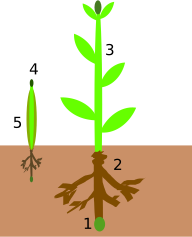
\includegraphics[width = 0.3\linewidth]{images/Spross.pdf}
	\caption{Grober Aufbau der Pflanze, links als Keimling, rechts als ausgewachsene Pflanze. Beschriftung: 1---Wurzelspitze, 2---Hauptwurzel mit Seitenwurzeln der ersten Ordnung, 3---Sprossachse, 4---Sprossspitze, 5---Koleoptil (Schutzorgan).}
\end{figure}

Am Anfang der Entwicklung einer Pflanze, wenn sie noch ein Keimling ist, wird sie von einem sehr sensiblen Schutzorgan, dem \emph{Koleoptil}, umgeben. Bei ausgewachsenen Pflanzen ist es nicht mehr vorhanden. 

Ausgewachsene Pflanzen bestehen aus einer Sprossachse, an dessen oberen Ende sich die Sprossspitze befindet. Am unteren Ende setzt die Hauptwurzel an, von der sich Seitenwurzeln, auch \emph{Adventivwurzeln} genannt, abzweigen. Am Ende der Hauptwurzel befindet sich die Wurzelspitze, hinter der sich die Streckungszone befindet.Die Streckungszone ist ein Bereich, in dem sich die Wurzelzellen durch Streckungswachstum vergrößern. Dadurch wird die Wurzelspitze weiter in die Erde vorgeschoben. An der Sprossspitze sowie an den Wurzelspitzen befinden sich \emph{Apikalmeristeme}, die eine Anhäufung sich teilender Zellen sind. Sie bilden Seitenzweige oder Blätter bei Sprossen und neue Wurzelzellen bei Wurzeln \parencite[1009--1011]{campbell}. 

\subsection{Arten des Gravitropismus}

Beim Gravitropismus, auch genannt Geotropismus, werden drei Bewegungsarten unterschieden: \emph{Positiv gravitrop},  \emph{negativ gravitrop} und \emph{transversalgravitrop}.

Positiv gravitrop bedeutet, dass das Wachstum der Organe, wie zum Beispiel Wurzeln, Rhizoide (wurzelähnliche Strukturen), Moose oder Farnprothallien, zur Schwerkraftquelle hin (nach unten zur Erdmitte) erfolgt. Negativ gravitrope Organe dagegen, wie Sprossen, Sporangienträger der Schimmelpilze der Gattung \emph{Mucor} oder Fruchtkörper mancher Pilze wachsen von der Schwerkraftquelle entgegengesetzt (nach oben). Diese zwei Wachstumsrichtungen werden auch als \emph{Orthogravitropismus} bezeichnet, da sie beide parallel zur Schwerkraft wachsen \parencite[546]{Jacob}.

Seitenwurzeln der ersten Ordnung (Nebenwurzeln, die von der Hauptwurzel entspringen) und zahlreiche Seitenzweige sowie Blätter wachsen \emph{transversalgravitrop}: entweder horizontal oder quer nach unten in einem bestimmten Winkel \parencite[449]{Strasburger}. 

\begin{figure}[H]
\centering 
 \includegraphics[width = 0.75\linewidth]{images/gravitrop_reagierende_Pflanze2.pdf}
 \caption{Gravitrop reagirende \emph{Arabidopsis thaliana} \parencite[5]{Masson2002}. Teilabbildung A zeigt den Zustand am Anfang, Teilabbildung B zeigt den Zustand nach vollzogener gravitropischer Reaktion. \label{gravitrop_reagierende_Pflanze}}
\end{figure} 
 
Legt man eine Pflanze quer, so werden sich Wurzeln und Spross krümmen, bis sie senkrecht stehen und wieder positiv bzw. negativ gravitrop wachsen \parencite[528]{Luettge}. Abbildung \ref{gravitrop_reagierende_Pflanze} zeigt diesen Prozess bei \emph{A. thaliana}. 

\section{Reizaufnahme bei Pflanzen}

Damit eine gravitrope Krümmung entstehen kann, werden zuvor Reize durch \emph{Statolithen} aufgenommen. Statolithen sind schwere Organelle in bestimmten Zellen des Sprosses sowie der Koleoptil-- und Wurzelspitzen; Abbildung \ref{Statolithen} zeigt ihren Aufbau und Wirkungsweise. Es handelt sich dabei meist um \emph{Amyloplasten}, die aus Stärke bestehen \parencite[530]{Luettge}.

\begin{figure}[H]
	\centering 
	\includegraphics[width = 0.75\linewidth]{images/Statolithen2.png}
	\caption{Statolithen \parencite[345]{Chen1999}. Teilabbildung a zeigt eine Mikroskopaufnahme von Statolithen bei \emph{A. thaliana}. Teilabbildungen b und c zeigen die gravitrope Wirkungsweise von Statolithen, die auf Umlagerung der Amyloplasten bei Veränderung des Schwerkraftvektors beruht. \label{Statolithen}}
\end{figure} 

Entscheidend ist der Stärkegehalt der Amyloplasten, denn ohne ihn geht die gravitrope Reaktionsfähigkeit verloren, wobei das Längenwachstum der Wurzeln weiterhin unbeeinflusst bleibt.
Die Stärke aus den Statolithenamyloplasten kann man durch experimentelle Eingriffe, zum Beispiel durch Kühlung, entfernen \parencite[452]{Strasburger}.

Die zahlreich vorhandenen Statolithen befinden sich in Zellen (\emph{Statocysten}), die die Graviperzeption ermöglichen. Kommen Statocysten in größeren Mengen vor, so bilden sie meist ein Gewebe, das als \emph{Statenchyme} bezeichnet wird. Diese Stärke enthaltenden Bereiche findet man in Wurzelspitzen und Innenzellschichten der Sprossachsen \parencite[501--502]{Nultsch}.  


Bei Einzelzellen, z.B einer \emph{Chara}-Rhizoide, werden Amyloplasten durch {\glqq Glanzkörper\grqq} ersetzt, die die Funktion der Statolithen übernehmen, da Einzelzellen keine Stärke enthalten. Diese in \emph{Vacuolen} liegenden Einschlusskörper besitzen einen hohes spezifisches Gewicht, da sie aus \ce{BaSO4} bestehen.

Die Streckung der Einzelzellen erfolgt nur durch Spitzenwachstum (einseitiges Wachstum der Zelle).
\emph{Dictyosomen} (flache, membranumhüllte Hohlräume in der Zelle) synthetisieren beim Spitzenwachstum Membran- und Zellwandbausteine für den Aufbau der wachsenden Rhizoidwand. Dieses Material wird in \emph{Vesikel} zur Wurzelspitze transportiert.
Wegen der Verlagerung der {\glqq Glanzkörper\grqq} auf die Unterseite
versperren sie den Weg für die Vesikeln. Sie müssen deswegen auf der Oberseite hindurch kommen, bewirken aber somit ein verstärktes Wandwachstum (positiver Gravitropismus) \parencite[453--454]{Strasburger}.
  
 \begin{figure}[H]
 	\centering 
 	\includegraphics[width = 0.75\linewidth]{images/Graviperzeption.jpeg}
 	\caption{Querlegen einer Wurzel der Kresse (\emph{Lepidium sativum}). Es erfolgt eine Graviperzeption, in der die Entlastung des Drucks der Membran des ER zu erkennen ist \parencite[533]{Luettge}. \label{Graviperzeption}}
 \end{figure} 
 
Bei Organen höherer Pflanzen ruhen Statolithen auf der Membran des \emph{endoplasmatischen Retikulums} (ER). Wird die Zelle gedreht, so wird auf einer Seite des Statocysten Druck ausgeübt, während die andere Seite entlastet wird. Wird das Organ um \ang{90} nach links gedreht, so wird die rechte Seite entlastet, und umgekehrt. Dies wird in der Abbildung \ref{Graviperzeption} genauer verdeutlicht. Dadurch erfolgt die Graviperzeption schneller, denn die Verlagerung der Wurzel hängt mit der Aufhebung des Statolithendrucks auf die Membran zusammen. Statolithen müssen dadurch nicht auf die Unterlage sinken, um dann von dort ein Signal über die veränderte Lage zu erzeugen \parencite[531--532]{Luettge}. 


\section{Signaltransduktion und differenzielles Wachstum}

Um eine Krümmung in Form von differenziellem Wachstum hervorzurufen, muss nach der Graviperzeption eine Signaltransduktion erfolgen, die die Änderung des Wachstumsverhaltens der Pflanze hervorruft. 

\subsection{Funktion des Calciums bei der Signaltransduktion}

Die Signalübermittlung durch den direkten Kontakt zwischen Amyloplasten und ER wird als \emph{gravisensorische Transduktion} bezeichnet.
Durch den Druck der Amyloplasten auf die ER-Membranen wird ein \ce{Ca^{2+}}-Efflux (das Austreten von Molekülen oder Ionen an der Zellmembran) aus dem ER verursacht.
Dadurch wird die lokale \ce{Ca^{2+}}-Konzentration im  \emph{Cytoplasma} erhöht. 
Bereits der Druck auf eine einzige ER-Zysterne reicht aus, um einen Efflux zu verursachen.

\subsection{Funktion des elektrischen Feldes bei der Signaltransduktion}

Ebenfalls wichtig bei der Signalumwandlung sind die Änderungen des elektrischen Feldes, welches die Wurzel umgibt.
Bei senkrecht stehenden Pflanzen wandern positiv geladene Ionen in die Wurzelspitze ein und treten im Bereich der Zellstreckzone wieder aus. Diese Ionenbewegung wird als \emph{apoplastischer Strom} bezeichnet; sie erzeugt das elektrische Feld, das die Wurzel umgibt. Dieses Feld ist mit einer hochempfindlichen Vibrationselektrode nachweisbar. 

Wird die Pflanze horizontal gelegt, so werden die Wurzeln gravitropisch gereizt. Dabei gelangen Protonen nur noch in die untere Flanke der Wurzelspitze hinein und auf der Oberseite hinaus, wodurch sich das elektrische Feld ändert \parencite[502--503]{Nultsch}. Dieses durch die Graviperzeption entstandene Signal kann nur in der Streckungszone hinter der Wurzelspitze aufgenommen werden. Kommt das Signal an, so setzt die Krümmung ein, indem die Flanken beginnen, ungleich zu wachsen. Damit ist feststellbar, dass der Perzeptions- und Reaktionsort getrennt sind.

\begin{figure}[H]
	\centering 
	\includegraphics[width = 0.4\linewidth]{images/newdiff.pdf}
	\caption{Flanken wachsen ungleich nach der Signaltransduktion. Linkes Bild: Flanken gleich groß (blau); rechtes Bild: unterschiedliche Größe der Flanken (rot und orange).}
\end{figure} 

Für diese Reaktion sind Eindauerzeiten des Reizes wichtig. Sie liegen meist zwischen 2 und 85 Minuten. Das dauert viel länger, als die kürzesten Reizeinwirkungen, die graviperzeptorisch noch wahrgenommen werden können und unter 30 Sekunden liegen. Somit wird bei jeder kleinen und kurzen Reizeinwirkung eine Vollführung der Krümmungsbewegung vermieden. Das ist wichtig für Pflanzen, um zum Beispiel eine gravitropische Reaktion auf eine Windeinwirkung zu verhindern \parencite[531]{Luettge}.

\subsection{Funktion der Auxine im Gravitropismus}

Die Ursache der Krümmung nach dem Signal ist die durch Schwerkraft hervorgerufene asymmetrische Verteilung des \emph{Auxins} \parencite[502--503]{Nultsch}.

Auxin ist ein Pflanzenhormon, das viele Funktionen besitzt. Dabei ist die Stimulierung der Zellstreckung (nur in niedriger Konzentration) und die Seiten- und Adventivwurzelbildung besonders wichtig. Andere Funktionen dieses Hormons sind die Regulierung der Fruchtentwicklung, die Verstärkung der Apikaldominanz, die Verzögerung des Blattfalls und die Förderung der Leitgewebedifferenzierung (hier und weiter Campbell und Reece 2009, S. 1118--1120).

Bei Pflanzen ist das natürliche Auxin die Indolessigsäure, aber alle Verbindungen, die zu einer Streckung von Koleoptilen führen, können als Auxin bezeichnet werden.

Beim Krümmungsprozess wird Auxin in einer Richtung direkt durch das \emph{Parenchymgewebe} (Gewebe, dessen Zellen nebeneinander liegen) transportiert: von der Sprossspitze längs der Sprossachse hin zur Basis. Dieser Transport wird als \emph{polarer Transport} bezeichnet und ist nicht von der Schwerkraft abhängig. Der Auxintransport geschieht durch Auxin-Transportproteine, die sich am basalen Zellenende befinden. Das Hormon wird zur Nachbarzelle am Apikalende transportiert.

Auxine werden im Apikalmeristem der Sprossachse synthetisiert. Von dort aus bewegen sie sich zur Streckungszone und stimulieren dabei das Zellwachstum. Diese Stimulierung ist jedoch nur möglich, wenn die Auxinkonzentration im Bereich zwischen $10^{-8}$ bis $10^{-4}$ \si{\mole\per\L} liegt. Bei höherer Konzentration kann Auxin die Zellstreckung durch Induktion der Ethylenbildung hemmen.

Bei der Wachstumsantwort der Zelle auf Auxin spielen Protonenpumpen eine entscheidende Rolle. Das Auxin stimuliert die Protonenpumpen der Plasmamembranen. Es werden Protonen herausgepumpt, wodurch das Membranpotenzial erhöht wird und der pH-Wert in der Zellwand gesenkt wird. Durch die Ansäuerung der Zellwand werden \emph{Expansine}, spezifische keilförmige Proteine, aktiviert, die die Zellwandstruktur auflockern, indem sie Wasserstoffbrückenbindungen zwischen Cellulosemikrofibrillen und anderen Zellwandbestandteilen lösen. Das erhöhte Membranpotenzial führt zur erhöhten Ionenaufnahme in die Zelle und damit zur Erhöhung des osmotischen Drucks (\emph{Turgor}). Da die Zellwand plastisch ist, kann sich die Zelle nun ausdehnen. 

Auch die Genexpression wird von Auxin sehr stark beeinflusst, sodass neue Proteine von den Zellen in der Streckungszone gebildet werden. Außerdem müssen Zellen mehr Cytoplasma und Zellwandmaterial synthetisieren, da das Wachstum aufrecht erhalten werden muss. Dies wird ebenfalls durch Auxin stimuliert \parencite[1118--1120]{campbell}.

Bei manchen Pflanzenarten (z.B. bei Sonnenblumen \emph{Helianthus} oder Bohnen \emph{Phaseolus}) spielt Auxin jedoch eine untergeordnete Rolle. Die Steuerung der Krümmung dieser Pflanzenarten übernehmen \emph{Gibberelline} \parencite[502--503]{Nultsch}.

\subsection{Funktion der Gibberelline im Gravitropismus}

Gibberelline sind, wie Auxin, Pflanzenhormone und besitzen mehrere Funktionen. Sie stimulieren die Sprossstreckung, beeinflussen Pollenentwicklung und sind für Pollenschlauch- und Fruchtwachstum sowie Samenentwicklung und Keimung verantwortlich. Außerdem bestimmen sie das Geschlecht in eingeschlechtigen Blüten und regulieren den Übergang von Jugendphasen zu Adultphasen. 

Bei der Zellstreckung wirken Gibberelline mit Auxin zusammen. Gibberelline aktivieren Enzyme, die die Zellwand auflockern und Expansinen den Eintritt in die Zellwand erleichtern \parencite[1122--1123]{campbell}.

Gravitropismus ist ein lebenswichtiges Resultat eines komplexen und zum Teil noch unerforschten Zusammenspiels von biologischen Akteuren \parencite[531]{Luettge}. Dennoch lässt sich die gesamte Kaskade mit einfachen Mitteln einleiten und kontrollieren, was zum experimentellen Teil der vorliegenden Arbeit führt. 

\chapter{Experimenteller Nachweis von Gravitropismus bei \emph{Lepidium sativum}}

Der experimentelle Teil der vorliegenden Arbeit befasst sich mit dem Nachweis von Gravitropismus bei Kresse (\emph{Lepidium sativum}) mit Einsatz eines dafür selbst konstruierten Klinostats. 

\section{Methoden}

\subsection{Pflanzen, Materialien und Geräte}

\subsubsection{\emph{Lepidium sativum} (Kresse)}

Für das Experiment wurde \emph{Lepidium sativum} (Kresse) ausgewählt. Sie ist eine schnellwüchsige Pflanze und kann auf jedem lockeren, durchlässigen Gartenboden wachsen. Es wurden Samen der Firma Kiepenkerl eingesetzt. 

Für die Anzucht wurden Anzucht-Quelltabs der Firma Windhager benutzt, die dafür sorgen, dass die Feuchtigkeit besser aufgenommen wird. Samen können dadurch schneller keimen und Wurzeln sich besser ausbilden, wodurch das Wachstum der Pflanze gefördert wird \parencite{Windhager}. 

\subsubsection{Klinostat}

Ein Klinostat ist ein Gerät, mit dem man Schwerkraft mittels Kreisbewegung simulieren kann. Ein Objekt auf einer sich drehenden Scheibe erfährt eine Schwerkrafteinwirkung in Form von Zentripetalkraft, wobei die Drehgeschwindigkeit die Stärke dieser Kraft bestimmt. Diesen Effekt macht man sich zunutze, um Schwerkraft in einer für eine Pflanze unnatürlichen Richtung zu simulieren. 

Für den Versuch wurde ein Klinostat selbstständig entwickelt und konstruiert. Abbildung \ref{Klinstat1} zeigt die Klinostatkonstruktion schematisch und erläutert den Aufbau, während Abbildung \ref{Klinostat2} den fertigen Versuchsaufbau demonstriert. 

\begin{figure}[H]
	\centering 
	\includegraphics[width = 0.75\linewidth]{images/drawing-1.pdf}
	\caption{Schematische Konstruktion des selbst gebauten Klinostats (seitliche Ansicht). 1---Befestigungsplatte (Holz, Dicke: 2cm), 2---Netzteil (Modell: MW1000GS, Eingang: 230V~50Hz 28W, Ausgang: 3-6-9-12V, 1000mA 12VA(max)), 3---Holzkeil, um die Drehachse des Motors um ca. \ang{15} senkrecht zur Ebene anzuheben, 4---Motorbefestigung, 5---Elektrogetriebemotor MFA/Como Drills 919D SERIES, single ratio gearbox 3000:1 (Untersetzung 3000:1), 4.5 - 15V DC, 6---Elektromotorwelle, 7---leere Blechdose mit Öffnung (wird mit einer Muffe an die Elektromotorwelle befestigt)\label{Klinstat1}.}
\end{figure} 


\begin{figure}[H]
	\centering 
	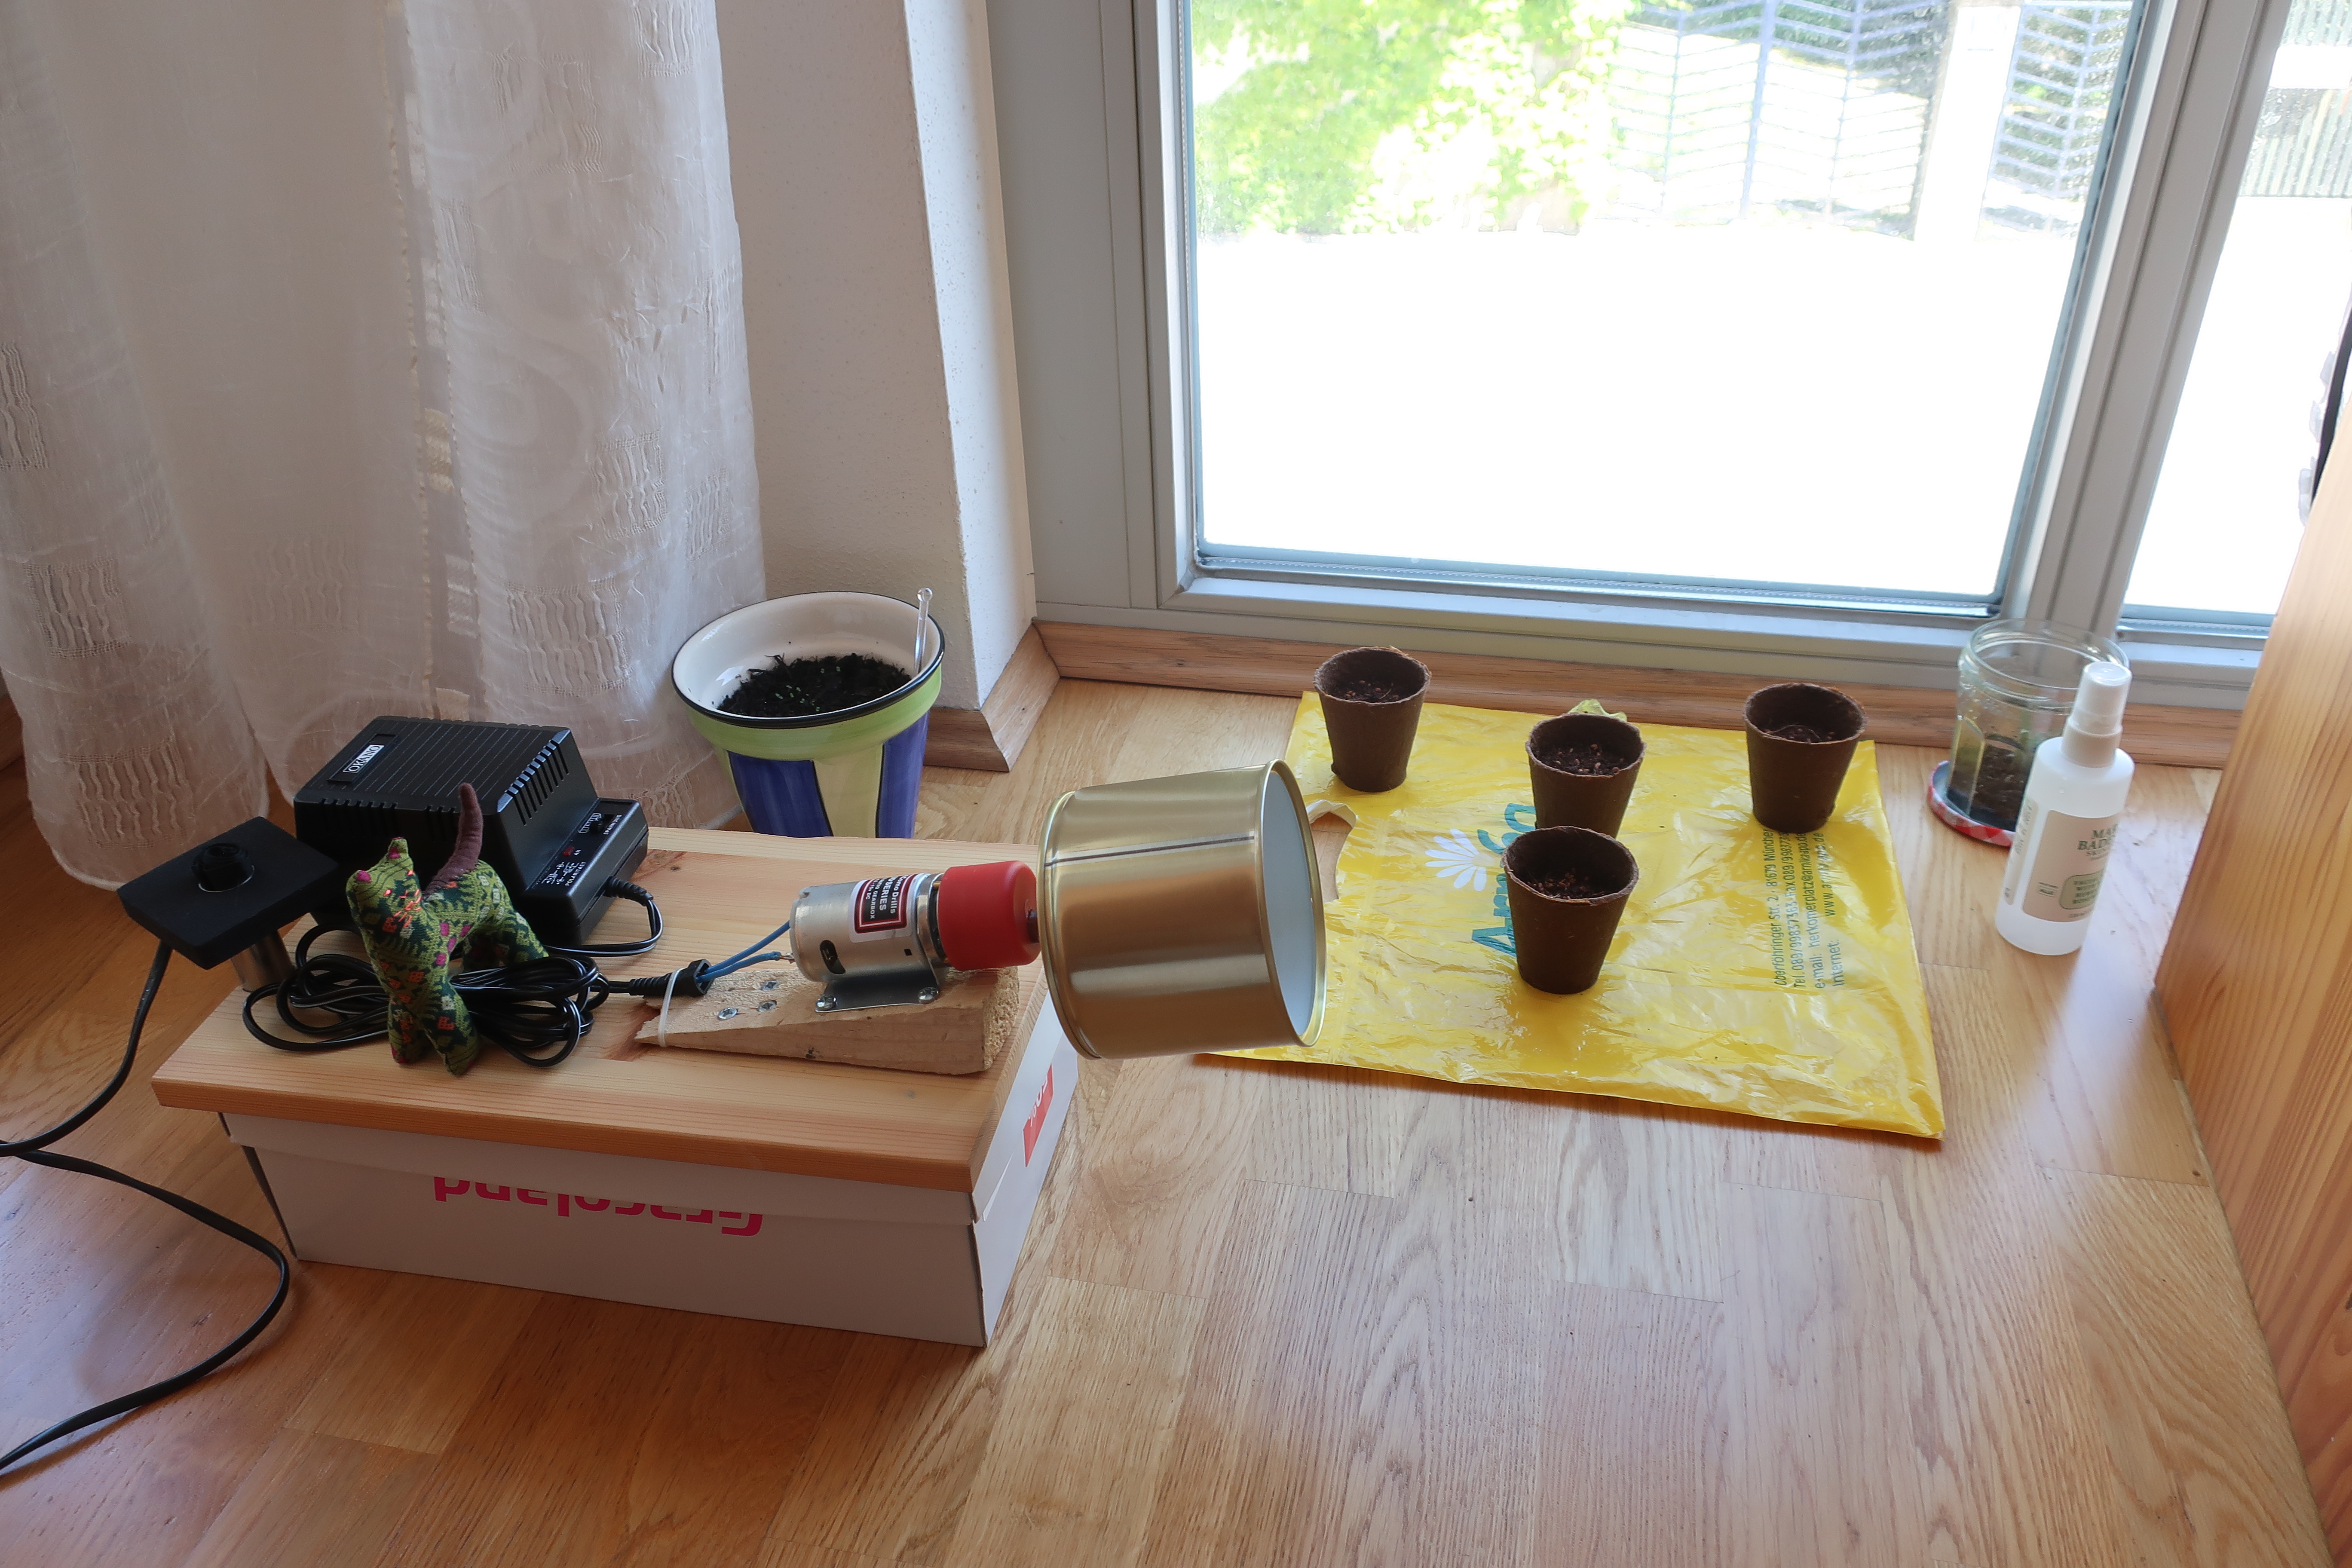
\includegraphics[width = 0.75\linewidth]{images/IMG_1044.JPG}
	\caption{Vorbereitung des Experiments und vollständig aufgebautes Klinostat.\label{Klinostat2}}
\end{figure}

\subsubsection{Weitere Materialien}

Für die Anzucht wurden vier gleich große Anzuchtbehälter (zylindrische Form, ca. 6 cm hoch und 6 cm im Durchmesser) eingesetzt. Aus einem Stoffstück wurde ein Säckchen gemacht, um es mit Erde zu füllen und bepflanzt am Klinostat zu befestigen. Außerdem wurde eine Plastiktüte, ein Messzylinder aus Plastik und diverse Gegenstände (z.B. Holzklotz) als Stütze für die Behälter verwendet. Für die Aufnahme des Experiments wurde eine Kamera (Canon PowerShot G9X II) verwendet.

\subsection{Versuchsmethodik}

Die Versuchsdurchführung gestaltet sich wie folgt. Es werden fünf kleine Vergleichspflanzengruppen von \emph{Lepidium sativum} vorbereitet, wobei jede Gruppe aus mindestens zwei Keimlingen bestehen soll. 

Nachdem die Pflanzen ausreichend angewachsen sind und gute Bodenhaftung haben, beginnt die Versuchsphase. Dabei wird: 

\begin{itemize}
	\item \textbf{Pflanzengruppe 1} als Kontrollgruppe im Anzuchttopf ohne besonderes Vorgehen klassisch (keine vertikale Neigung, keine Nutzung des Klinostats) gezüchtet
	\item \textbf{Pflanzengruppe 2} im Säckchen am Klinostat unter Einwirkung von Zentripetalkraft gezüchtet 
	\item \textbf{Pflanzengruppe 3} im Anzuchttopf kopfüber gezüchtet
	\item \textbf{Pflanzengruppe 4} im Anzuchttopf horizontal am Boden gezüchtet
	\item \textbf{Pflanzengruppe 5} im Anzuchttopf mit Winkel zum Boden von ca. \ang{45} gezüchtet 
\end{itemize}

Somit soll der Vergleich der verschiedenen gravitropen Reize und der entsprechenden Wachstumsänderung ermöglicht werden. Die Versuche werden gestaffelt: zunächst wird das Klinostat-Experiment durchgeführt (2 Tage), anschließend das Ausrichtungs-Experiment (2 Tage). Es wird also die gravitrope Wirkung des Klinostats und der räumlichen (Neu-)Ausrichtung getrennt untersucht. 

Die Versuchsansätze werden regelmäßig kontrolliert und fotografisch aufgezeichnet. Es werden stellenweise auch Videoaufzeichnungen vom Versuchsaufbau und -ablauf angefertigt, die Videoaufnahmen werden hier jedoch nicht weiter besprochen bzw. ausgewertet (sie liegen der vorliegenden Arbeit als Videodateien dennoch anbei). 

\section{Durchführung und Ergebnisse}

\subsection{Vorbereitung (Versuchstag 1, 28.05.2018)}

Das Experiment wird vorbereitet. Als Versuchsort wird der Fußboden vor einem Fenster ausgewählt, wo eine Plastiktüte ausgebreitet wird, um Schmutz auf dem Boden zu vermeiden. Die vier Anzuchtbehälter (Gruppe 1 und Gruppen 3--5) werden mit Anzuchterde gefüllt (2/3 der Becher) und mit jeweils 20 Samen bestückt. Das Säckchen (Gruppe 2) wird ebenfalls mit Anzuchterde befüllt und mit drei Samen versehen. 

\subsection{Ankeimen (Versuchstage 2--4, 29.--31.05.2018)}

Nach der Einpflanzen werden die Pflanzen täglich mit Wasser versorgt (jeweils 20 mL), Bedingungen wie Licht und Wärme werden, soweit möglich, konstant gehalten (aber nicht gesondert gemessen). Veränderungen der Pflanzen werden beobachtet und notiert. Als Voraussetzung für die weitere Durchführung des Versuchs müssen zunächst Keime in allen Anzuchttöpfen vorhanden sein und stabil wachsen. Diese erste Phase des Versuchs dauert 2 Tage und verläuft wie folgt. 

\subsubsection{Versuchstag 2 (29.05.2018)} 

Die Samen keimen in allen Gruppen. 

\subsubsection{Versuchstag 3 (30.05.2018)} 

Sprossen wachsen gleichmäßig um ca.\,2 cm (keine Blätter). Zu diesem Zeitpunkt sind die Sprösslinge nicht geeignet, da die Haftung nicht ausreicht. 

\subsubsection{Versuchstag 4 (31.05.2018)} 

Sprösslinge haben Blätter gebildet und sind geeignet für das Experiment, da ihre Bodenhaftung nun stabil ist. Abbildung \ref{amanfang} zeigt beispielhaft eine der Behälter-Pflanzengruppen, die alle vergleichbar angewachsen sind. 

\begin{figure}[H]
	\centering 
	\includegraphics [width =.75\linewidth]{images/IMG_1104.JPG}
	\caption{Sprösslinge im Behälter am Anfang des Versuchs.\label{amanfang}}
\end{figure} 

\subsection{Klinostat-Experiment mit Pflanzengruppe 2 (Versuchstage 4--5, 31.--01.06.2018)} 

An den Versuchstagen 4--5 wird das Klinostat-Experiment mit Pflanzengruppe 2 durchgeführt. 

\subsubsection{Versuchstag 4 (31.05.2018)} 

Das Säckchen mit Gruppe 2 wird am Klinostat befestigt. Danach wird das Klinostat gestartet und eine Umdrehungsgeschwindigkeit von einer Umdrehung pro Minute eingestellt. Der Versuch beginnt um 12:45 Uhr (Abbildung \ref{Foto 1}) und wird um 15:45 beendet, da die Sprösslinge gravitrop reagiert haben (Abbildung \ref{Foto 2}). 

\begin{figure}[H]
	\centering
	\begin{subfigure}[b]{0.44\textwidth}
		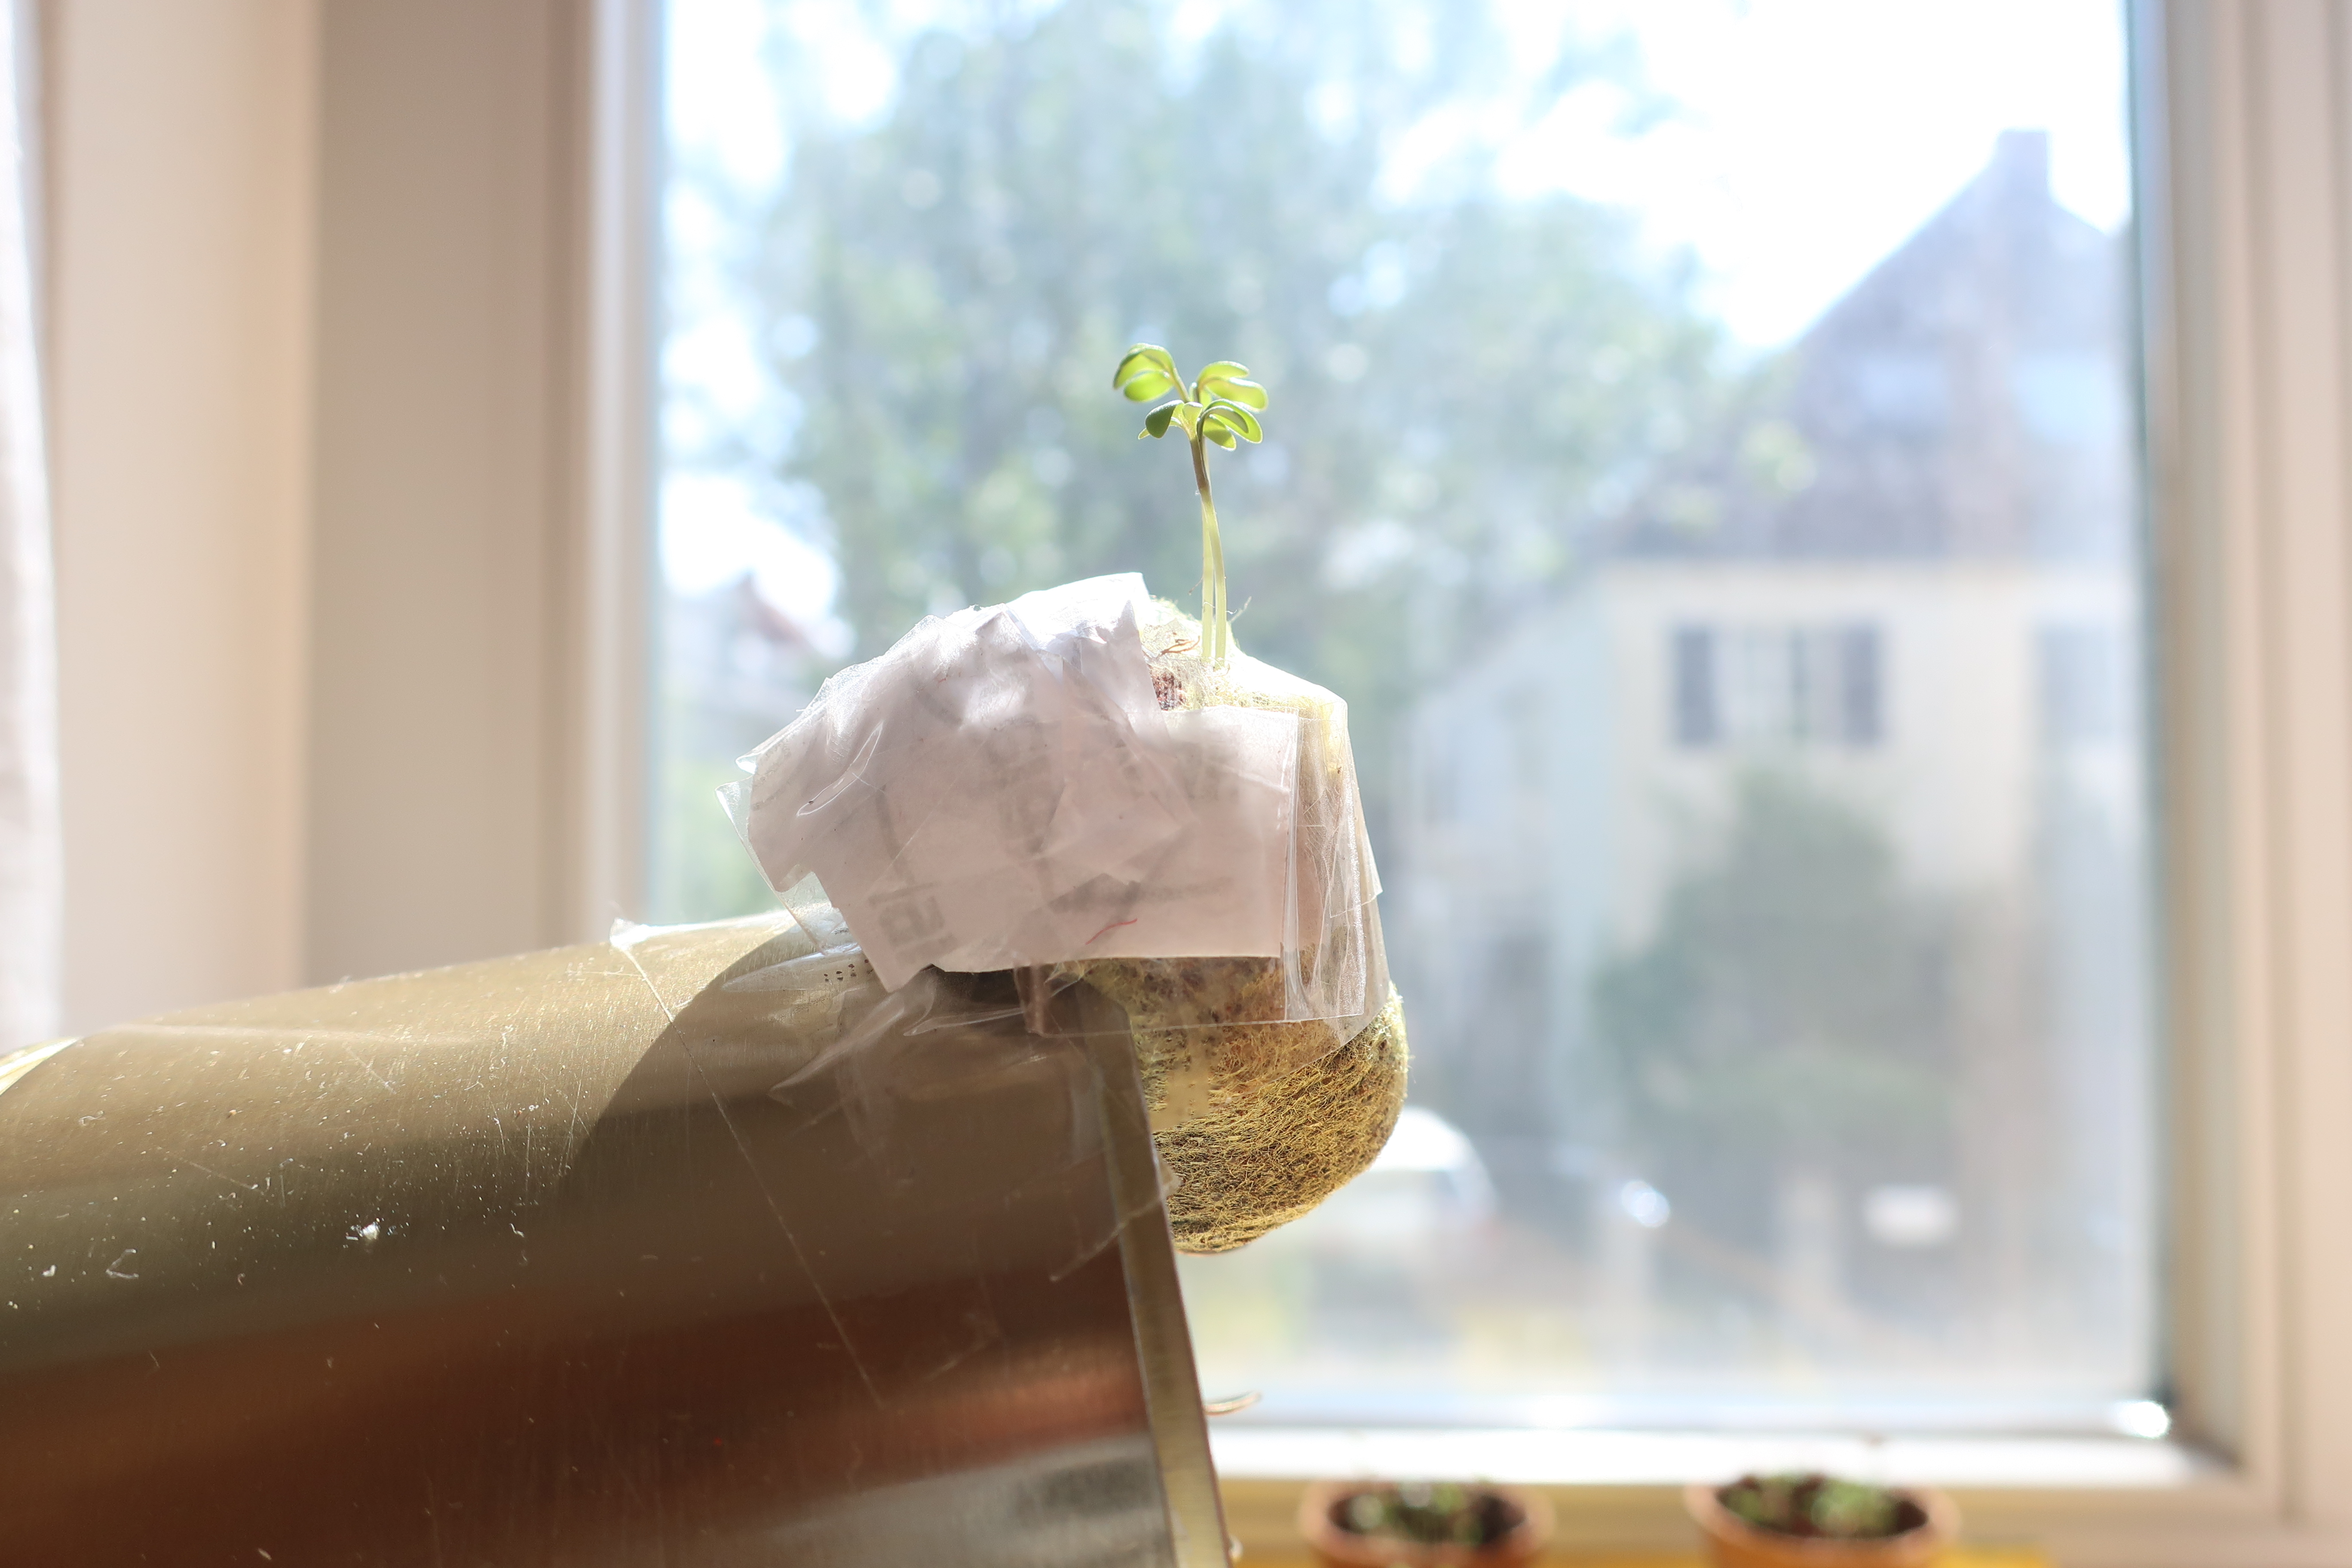
\includegraphics[width=\textwidth]{images/IMG_1083.JPG}
		\caption{Sprossen vor Beginn des Klinostat-Experiments.\label{Foto 1}}
		
	\end{subfigure}
	~ %add desired spacing between images, e. g. ~, \quad, \qquad, \hfill etc. 
	%(or a blank line to force the subfigure onto a new line)
	\begin{subfigure}[b]{0.44\textwidth}
		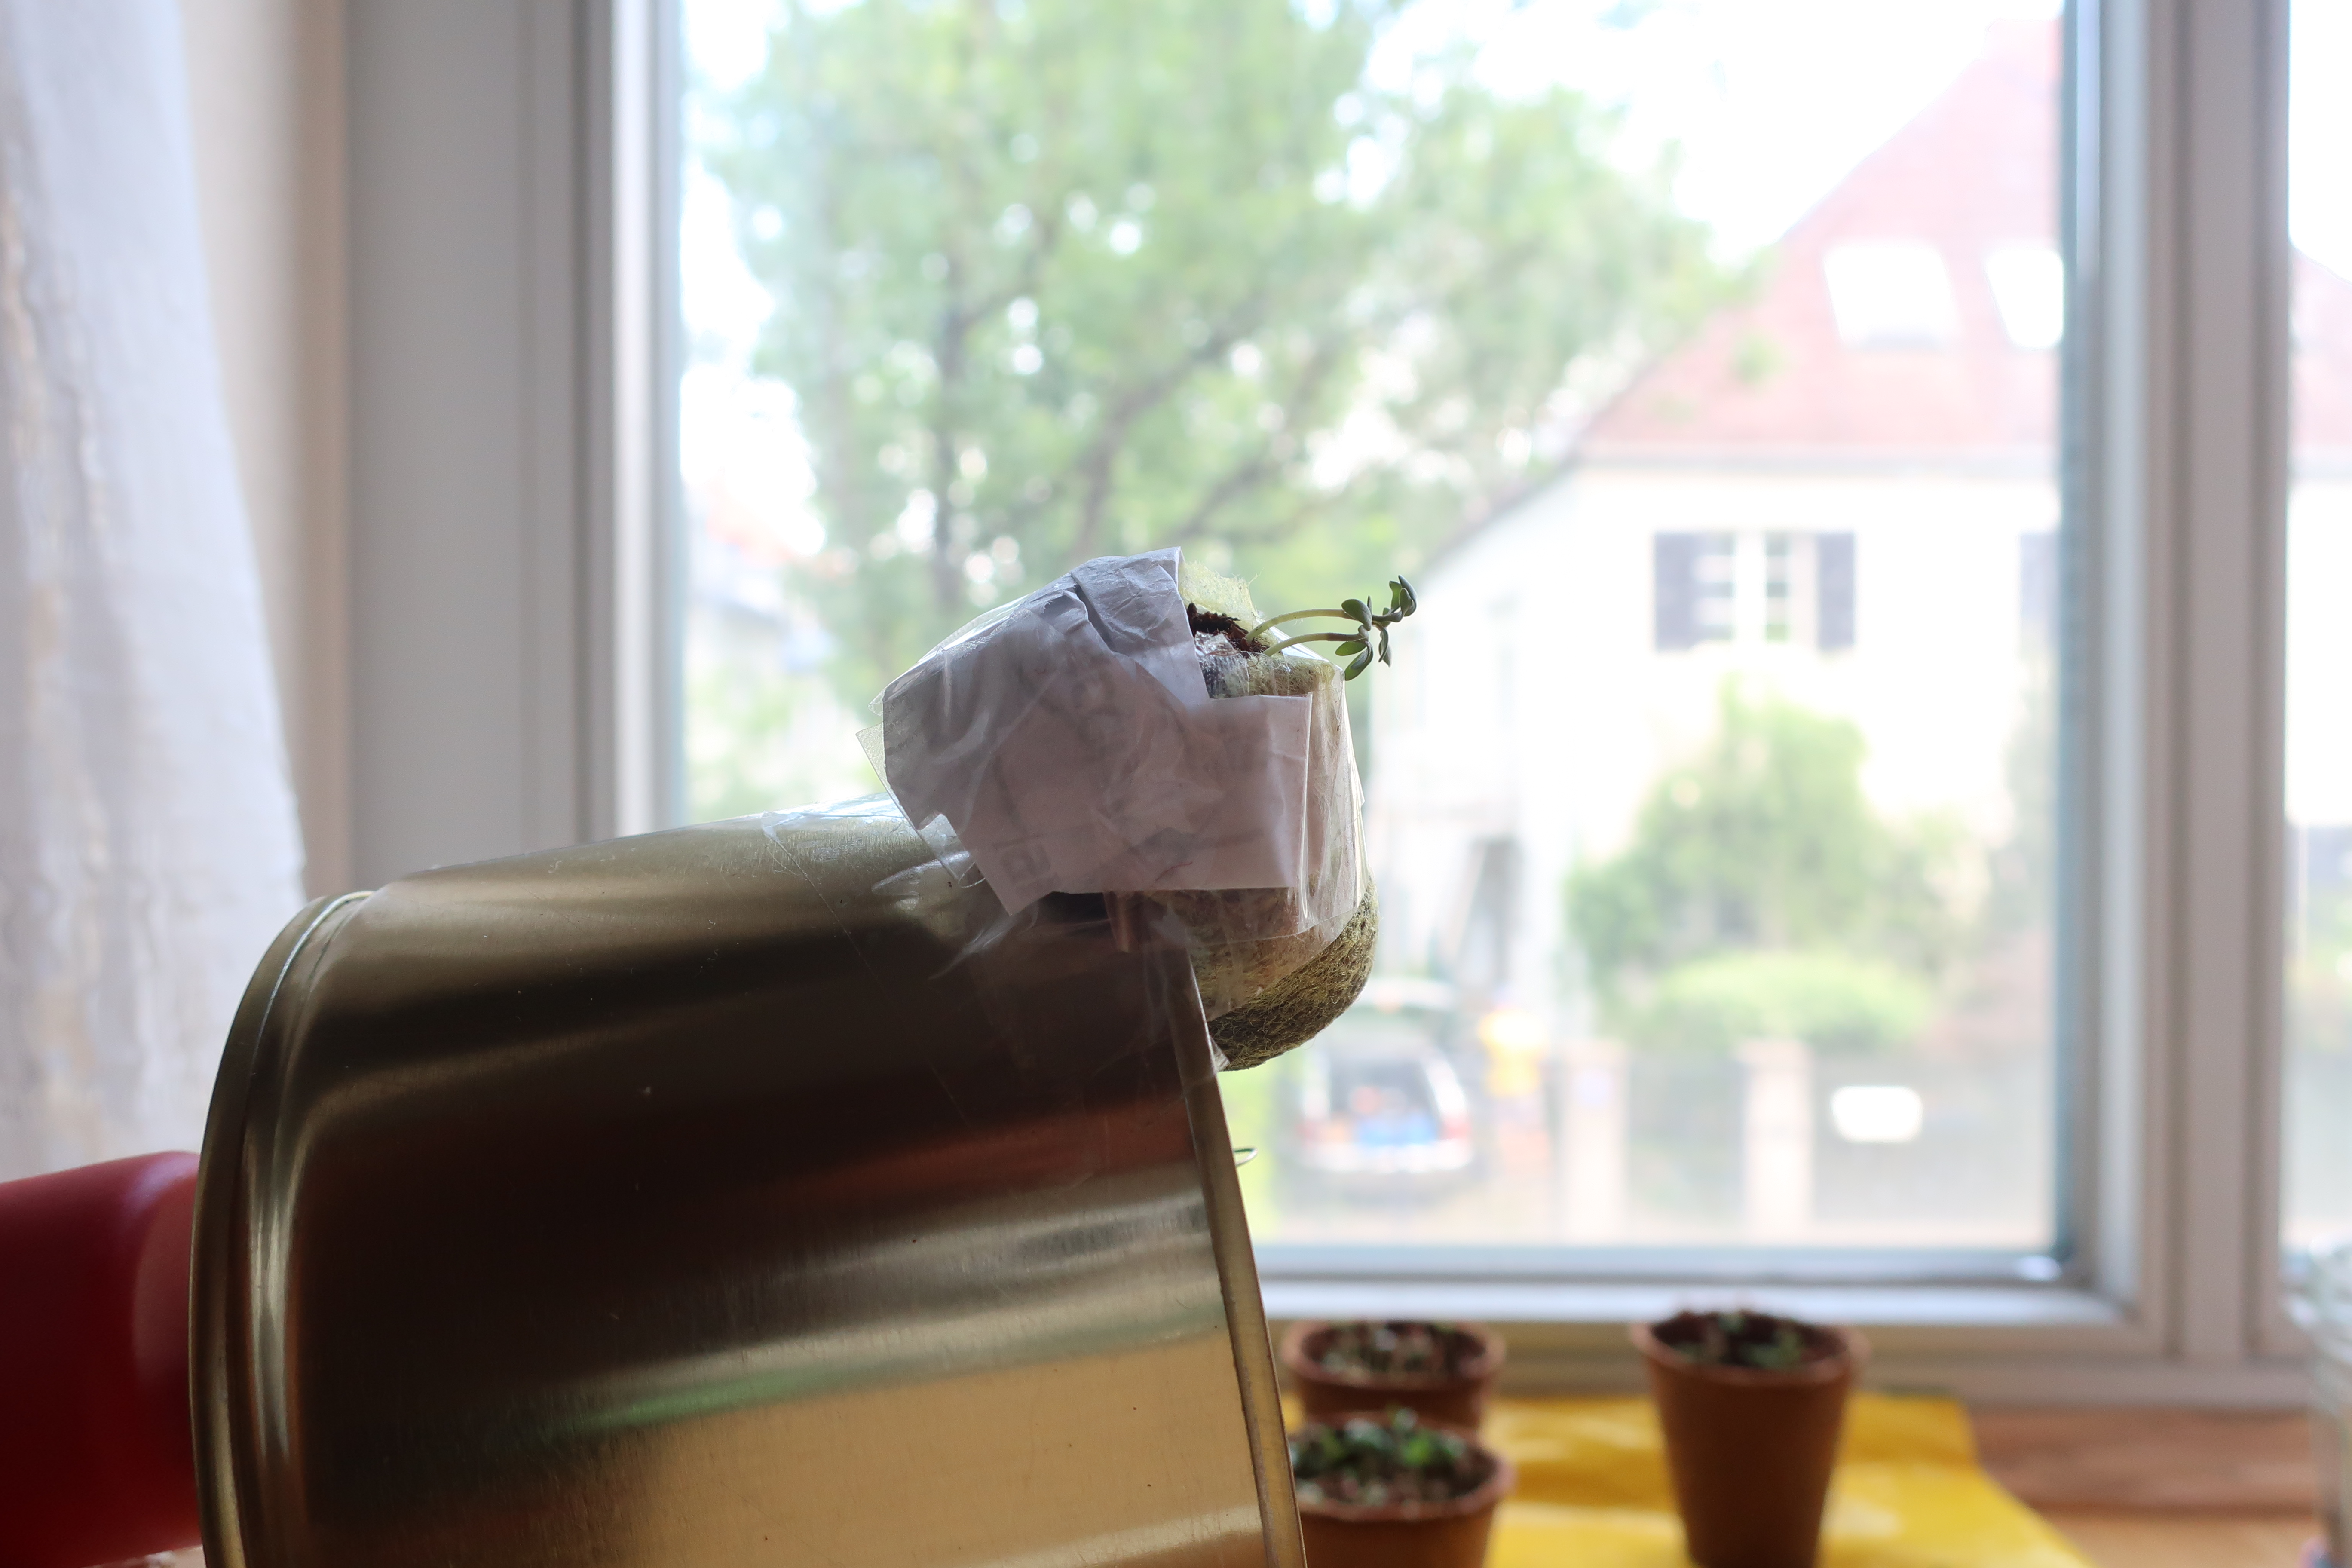
\includegraphics[width=\textwidth]{images/IMG_1073.JPG}
		\caption{Sprossen nach Abschalten des Klinostats.\label{Foto 2}}
	\end{subfigure}
	\caption{Klinostat-Experiment, Pflanzengruppe 2.\label{Foto 2}}
\end{figure}

\subsubsection{Versuchstag 5 (01.06.2018)} 

Über Nacht haben sich die Pflanzen wieder aufgerichtet, somit ist eine Wiederholung des Versuchs mit Gruppe 2 möglich und der Versuch wird analog zum Versuchstag 4 um 11:45 gestartet. Allerdings wird um 12:53 festgestellt, dass das Klinostat mittlerweile defekt ist. Die Pflanzen der Gruppe 2 haben sich jedoch bereits sichtbar nach oben gebogen. Die Drehzeit betrug ca. 1 Stunde und 8 Minuten.

\subsection{Ausrichtungs-Experiment mit Pflanzengruppen 3--5 (Versuchstage 6--7, 02.--03.06.2018)} 

An den Versuchstagen 6 und 7 wird das Ausrichtungs-Experiment mit Gruppen 3--5 durchgeführt, bei dem die drei Behälter in verschiedenen Positionen gebracht werden: Gruppe 3 parallel zum Boden, Gruppe 4 kopfüber und Gruppe 5 im Winkel von ca. \ang{45}.

\subsubsection{Versuchstag 6 (02.06.2018)} 

Langsames Wachstum der Gruppen 3--5. 

\subsubsection{Versuchstag 7 (03.06.2018)} 

Die Sprösslinge der Gruppen 3--5 zeigen ebenfalls gravitropes Verhalten, etwas weniger ausgeprägt, als Gruppe 2 im Klinostat-Experiment. Abbildungen \ref{A3}, \ref{A4} und \ref{A5} zeigen die Sprossen der Gruppen 3--5 jeweils vor und nach dem Ausrichtungsexperiment.  

% \begin{figure}[H]
% 	\centering 
% 	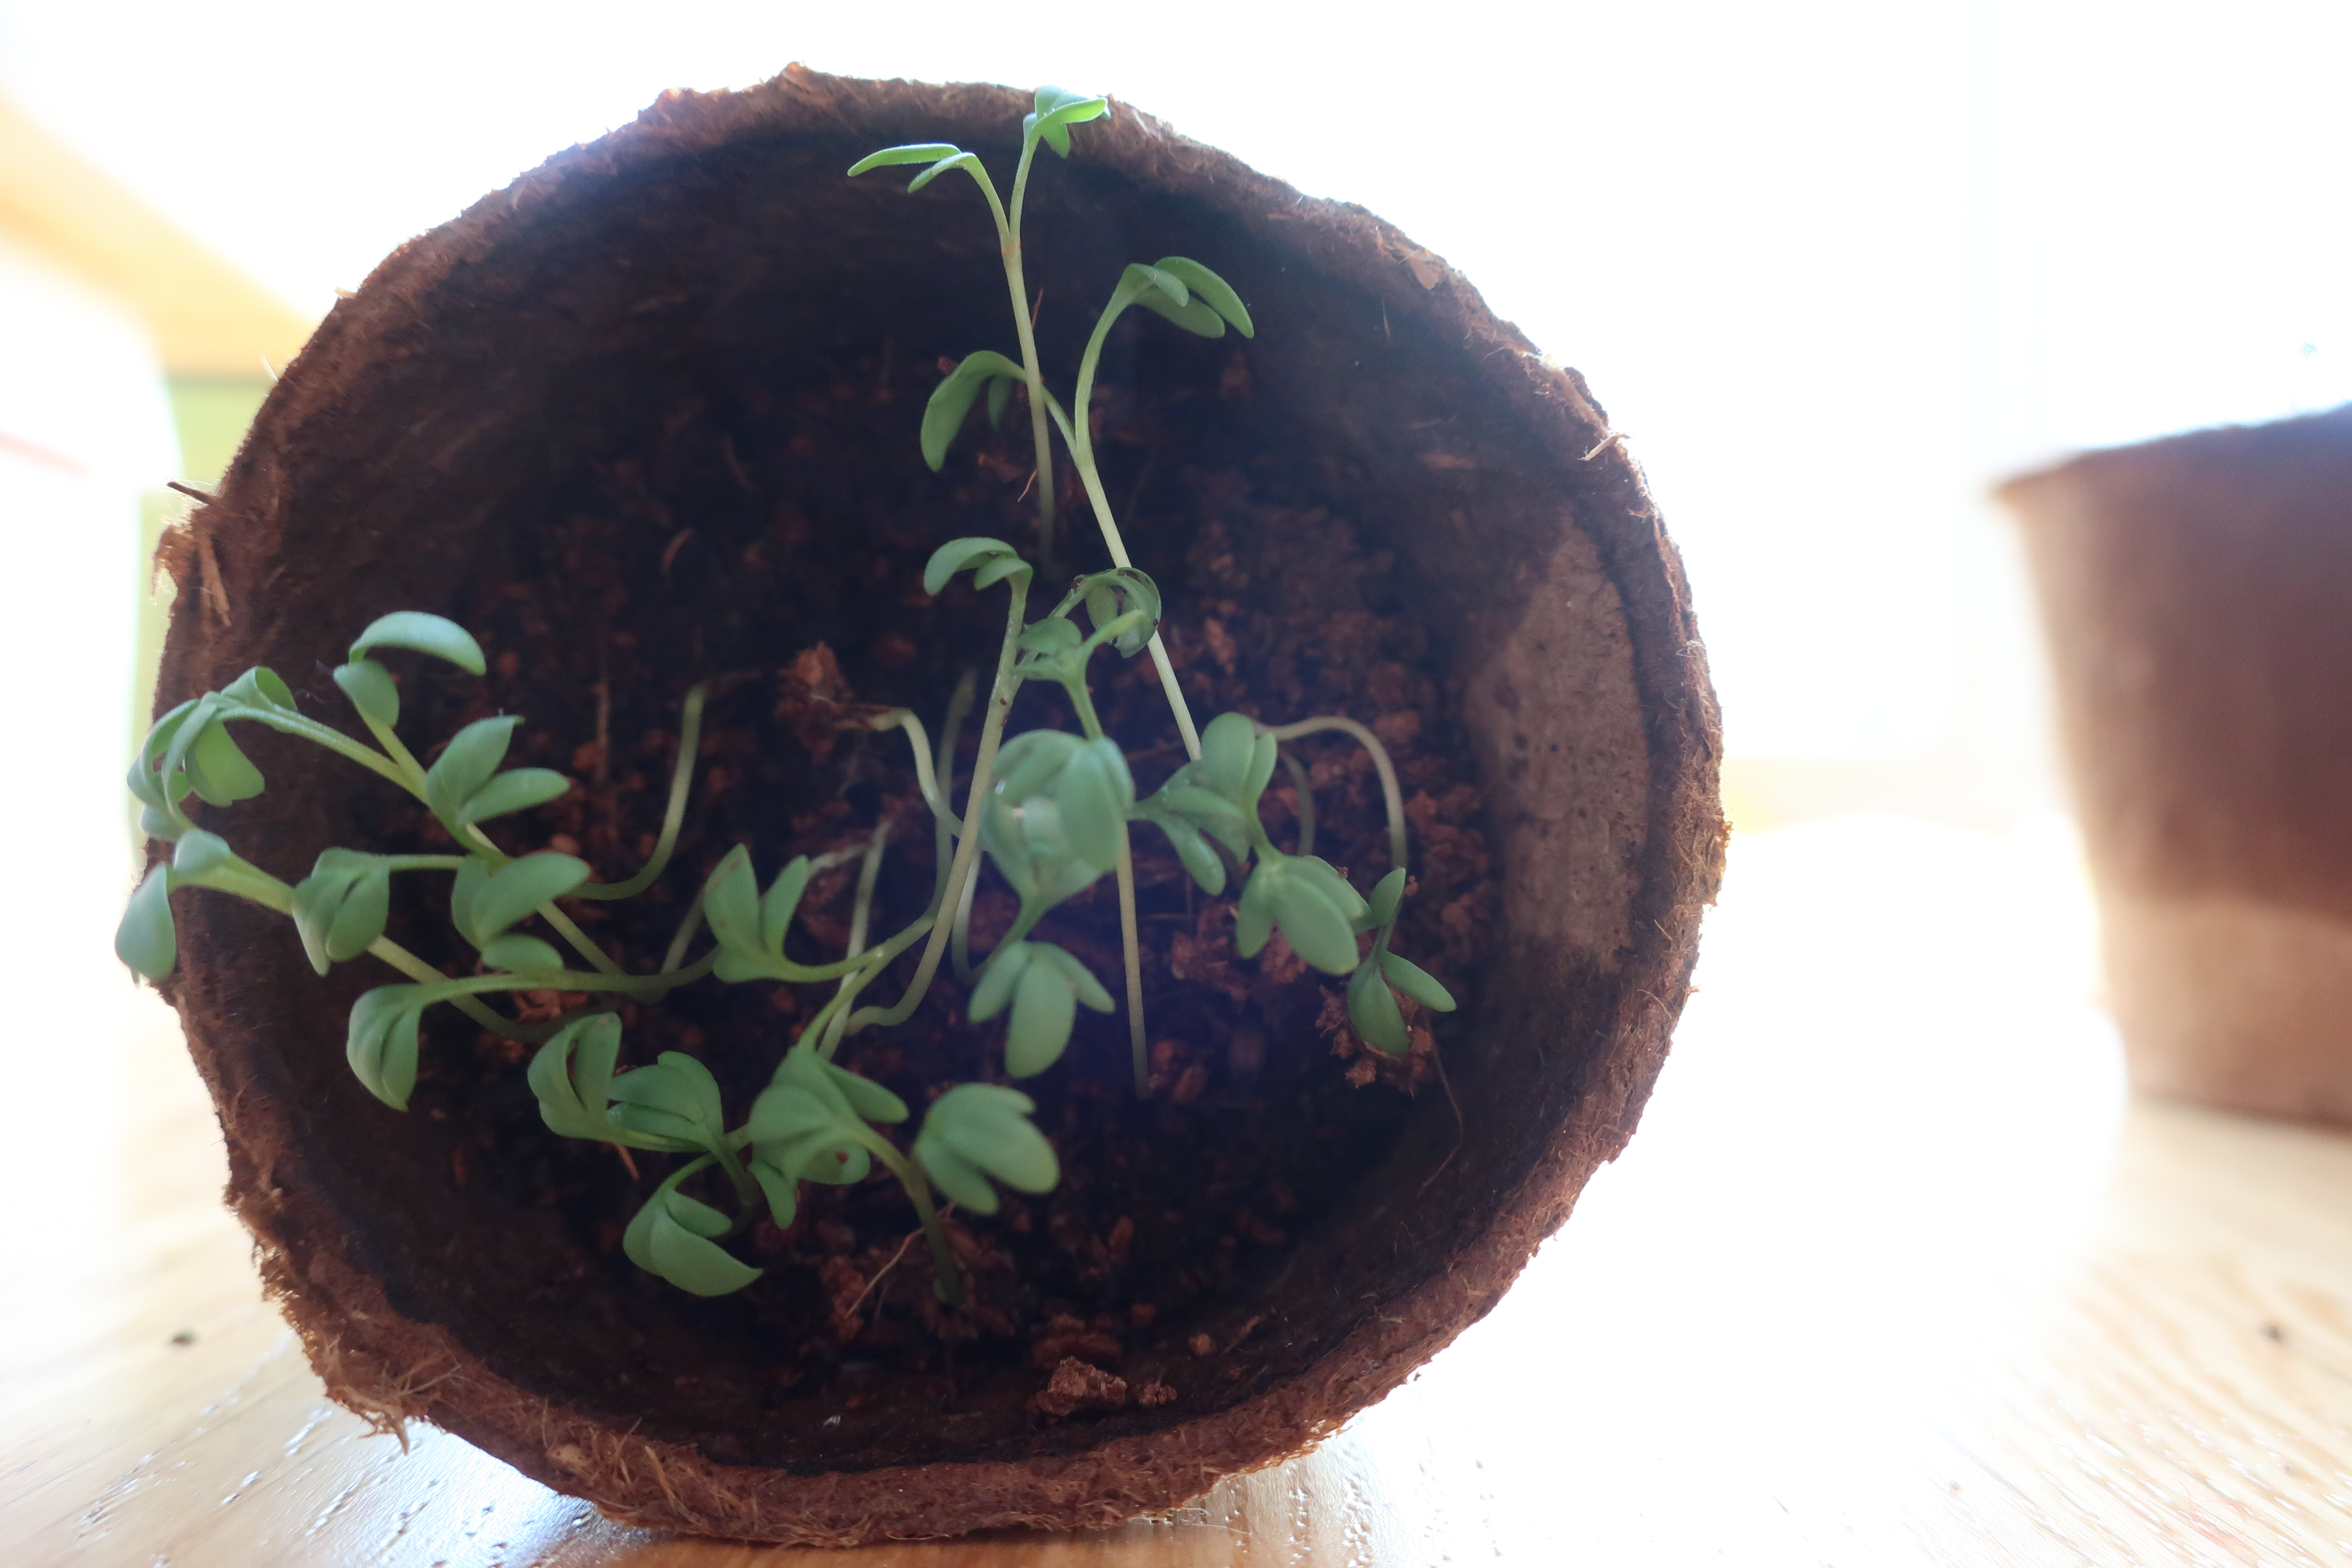
\includegraphics [width =.5\linewidth]{images/IMG_1120.JPG}
% 	\caption{Sprösslinge der Gruppe 4 am Ende des Versuchs\label{Foto 5}.}
% \end{figure} 

\begin{figure}[H]
	\centering
	\begin{subfigure}[b]{0.44\textwidth}
		\includegraphics[width=\textwidth]{images/A3/IMG_1102.JPG}
		\caption{Sprossen vor Neuausrichtung.\label{A31}}
		
	\end{subfigure}
	~ %add desired spacing between images, e. g. ~, \quad, \qquad, \hfill etc. 
	%(or a blank line to force the subfigure onto a new line)
	\begin{subfigure}[b]{0.44\textwidth}
		\includegraphics[width=\textwidth]{images/A3/IMG_1398.JPG}
		\caption{Sprossen am Versuchstag 7.\label{A37}}
	\end{subfigure}
	\caption{Ausrichtungs-Experiment, Pflanzengruppe 3 (kopfüber).\label{A3}}
\end{figure}

\begin{figure}[H]
	\centering
	\begin{subfigure}[b]{0.44\textwidth}
		\includegraphics[width=\textwidth]{images/A4/IMG_1104.JPG}
		\caption{Sprossen vor Neuausrichtung.\label{A41}}
		
	\end{subfigure}
	~ %add desired spacing between images, e. g. ~, \quad, \qquad, \hfill etc. 
	%(or a blank line to force the subfigure onto a new line)
	\begin{subfigure}[b]{0.44\textwidth}
		\includegraphics[width=\textwidth]{images/A4/IMG_1396.JPG}
		\caption{Sprossen am Versuchstag 7.\label{A47}}
	\end{subfigure}
	\caption{Ausrichtungs-Experiment, Pflanzengruppe 4 (horizontal).\label{A4}}
\end{figure}

\begin{figure}[H]
	\centering
	\begin{subfigure}[b]{0.44\textwidth}
		\includegraphics[width=\textwidth]{images/A5/IMG_1101.JPG}
		\caption{Sprossen vor Neuausrichtung.\label{A51}}
		
	\end{subfigure}
	~ %add desired spacing between images, e. g. ~, \quad, \qquad, \hfill etc. 
	%(or a blank line to force the subfigure onto a new line)
	\begin{subfigure}[b]{0.44\textwidth}
		\includegraphics[width=\textwidth]{images/A5/IMG_1397.JPG}
		\caption{Sprossen am Versuchstag 7.\label{A57}}
	\end{subfigure}
	\caption{Ausrichtungs-Experiment, Pflanzengruppe 5 (diagonal).\label{A5}}
\end{figure}

Die Planzengruppe 1 (Kontrollgruppe) zeigt in den 7 Versuchstagen, wie erwartet, normales gerades Wachstum. 

\section{Diskussion}

Die Versuchsreihe, bestehend aus Klinostat-Experiment und Ausrichtungs-Experiment, zeigt deutlich die gravitrope Reaktion von \emph{Lepidium sativum}, sowohl auf Drehung, als auch auf veränderte räumliche Position. Insofern ist der experimentelle Teil insgesamt als gelungen zu betrachten. 

Die Konstruktion und der Einsatz vom Klinostat lassen sich als einer der Kernpunkte der vorliegenden Arbeit als durchaus erfolgreich bezeichnen, trotz der kleineren Panne am Versuchstag 5.

\paragraph{Abhängigkeit des gravitropen Effekts von verschiedenen Faktoren }

Aufgrund der unterschiedlichen Reaktionsstärke unterhalb der Pflanzengruppen 2--5 lässt sich vermuten, dass der gravitrope Effekt und damit die Krümmungsstärke von verschiedenen Faktoren abhängt: 

\subparagraph{Sprosslänge} Die Sprosslänge der Gruppe 2 unterschied sich von der Sprosslänge der Gruppen 3--5 aufgrund der zeitlichen Staffelung der Experimente. Es lässt sich notieren, dass der gravitrope Reiz bei Kressepflanzen, deren Sprosslänge unter 3 cm beträgt, die Krümmung innerhalb von 1-3 Stunden hervorruft, während bei Sprösslingen über 3 cm Länge die Krümmung über 24 Stunden erfolgt. Als mögliche Erklärung lässt sich folgende Hypothese aufstellen: da die Sprösse jünger und kleiner sind, wachsen sie vergleichsweise schneller, somit ist auch die gravitrope Reaktion zügiger. 

\subparagraph{Stärke des Reizes} Die Krafteinwirkung war verschieden unter den Gruppen, ebenso wie die Krümmungsstärke. 

\subparagraph{Übermäßiger Reiz} Übermäßiger Reiz zeigt eventuell eine Gegenwirkung: Pflanzengruppe 3 (kopfüber) zeigt keine extreme gravitropische Reaktion, trotz der totalen Umkehr des Schwerkraftvektors. 

\subparagraph{Lichteinwirkung, Reizkonkurrenz} In den Versuchen haben sich Pflanzen nicht komplett senkrecht gerichtet, sondern mehr zum Licht gewandt. Das liegt daran, dass Pflanzen sich immer zum Licht richten, um Photosynthese zu betreiben. Dies zeigt deutlich, dass Gravitropismus und Phototropismus in Konkurrenz stehen und einander beeinflussen können.

\subparagraph{Unberücksichtigte Faktoren} Eventuelle unberücksichtigte Faktoren, die hier unbekannt geblieben sind, könnten auch Einfluss genommen haben. Hierzu könnten gehören:

\begin{itemize}
\item Schwankungen in pflanzlichen Hormonen
\item unterschiedliche Samen
\item unterschiedliche initiale Wachstumsphasen
\item Umweltfaktoren wie Druck, Temperatur und Feuchtigkeit
\item Einflüsse durch das Nährmedium 
\end{itemize}

\paragraph{Verbesserungsmöglichkeiten}

Deutliches Verbesserungspotential besteht bei den fotografischen Aufnahmen. Beleuchtung und Kameraarbeit könnten besser abgestimmt werden, vor allem aber wären konsistentere Aufnahmebedingungen nützlich gewesen, um besser zwischen den Pflanzengruppen vergleichen zu können. Die vorliegenden Aufnahmen erlauben lediglich eine subjektive qualitative Auswertung. Dieses Defizit lässt sich auf den Mangel an Fotografie-Erfahrung zurückführen. 

Ebenso wären im Rückblick genaue Messungen der Winkel und Längen der Sprösse mit fotografischem Beleg sinnvoll, um quantitative Datenvergleiche zu ermöglichen. 

\chapter{Fazit und Ausblick}

Die durchgeführten Versuche zeigen deutlich den gravitropen Effekt bei \emph{Lepidium sativum}. Sie zeigen auch, dass mehrere Faktoren diesen Prozess beeinflussen können. Es ist ersichtlich, dass der Prozess des Gravitropismus in drei Schritten erfolgt. Zuerst erfolgt die Reizaufnahme, dann die Signalübermittlung und zuletzt die Krümmung. Zwischen diesen Schritten wirken biologische Mechanismen, die teilweise noch nicht ganz geklärt sind, aber uns helfen den Gravitropismus besser zu verstehen. 

Aus den Resultaten der vorliegenden Arbeit bieten sich diverse weiterführende Forschungsansätze an: 

\begin{itemize}
	\item Der Versuch ließe sich verbessern, indem eine konstante neutrale Beleuchtung sichergestellt wird, um die Einwirkung des phototrophen Effekts zu minimieren. 
	\item Die Reizabhängigkeit des gravitropen Effekts könnte quantifiziert werden. 
	\item Die Abhängigkeit des gravitropen Effekts von anderen Faktoren und Umweltbedingungen, wie in der Diskussion bereits erwähnt, kann untersucht werden. 
	\item Der Einfluss der Pflanzenwahl ließe sich durch Wiederholung des Versuchs mit mehreren anderen Pflanzenarten ausmitteln. 
	\item Die mechanische Stärke des gravitropen Effekts könnte mit entsprechend empfindlicher Ausrüstung gemessen werden. 
	\item Die in der Diskussion aufgestellte Hypothese über die schnellere gravitrope Reaktion von jüngeren Pflanzen ließe sich eventuell prüfen, indem man bei älteren Pflanzen unter Einwirkung eines starken gravitropen Reizes durch Hormonzugabe die Wachstumsrate künstlich beschleunigt und kontrolliert, ob und inwiefern sich die gravitrope Reaktionszeit ändert (ein Ausbleiben dieser Änderung wäre ein Indiz dafür, die Hypothese als widerlegt zu betrachten). 
\end{itemize}

Die Wichtigkeit der Erforschung von Gravitropismus ergibt sich klar aus seiner Allgegenwärtigkeit in der Welt der Pflanzen, aber auch beispielsweise in einem ökonomischen Zusammenhang, wie im Bereich der Landwirtschaft\parencite[343]{Chen1999}. Zu den Forschern, die einen bedeutenden Beitrag zur Erklärung des Phänomens des Gravitropismus geleistet haben, gehören Markus Braun, Zygmunt Hejnowicz, Rujin Chen, Elizabeth Rosen und Patrick H. Masson.


\printbibliography

\listoffigures

\chapter {Schlusserklärung}

Ich erkläre, dass ich die Seminararbeit ohne fremde Hilfe angefertigt und nur die im Literaturverzeichnis angeführte Quellen und Hilfsmittel benützt habe.
\\
\\
\\
\\
\\
\setlength\tabcolsep{0pt}\noindent\hspace{-.2mm}\begin{tabular}{p{.2\textwidth} p{.01\textwidth} p{.02\textwidth} p{.2\textwidth} p{.10\textwidth} p{.47\textwidth}}
	\Dotfill & \hfill, & & \Dotfill &  & \Dotfill \\ 
 \hspace{.2mm}Ort & & &  \hspace{.2mm}Datum &  &  \hspace{.2mm}Unterschrift des Schülers\,/\,der Schülerin \\
\end{tabular}

\end{document}
